\documentclass[tikz, border=4pt]{standalone}
\usepackage{tikz}
\usetikzlibrary{patterns.meta}
\begin{document}
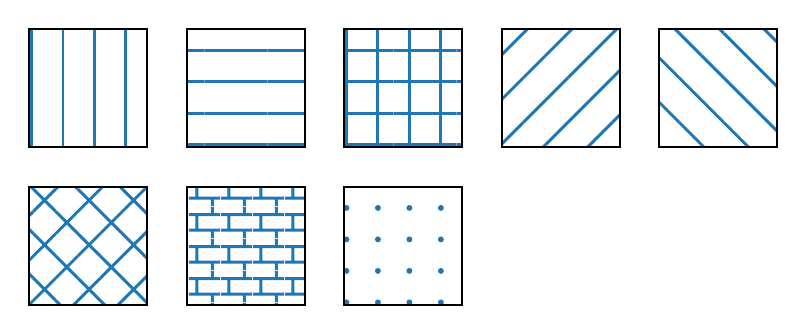
\begin{tikzpicture}[x=1cm, y=1cm]
  \definecolor{tdc1}{HTML}{1F77B4}
  \pgfdeclarepattern{name=tdbricks0, parameters={}, bottom left={\pgfpoint{0pt}{0pt}}, top right={\pgfpoint{11.38pt}{11.38pt}}, tile size={\pgfpoint{11.38pt}{11.38pt}}, code={\pgfsetlinewidth{1.07pt}\pgfpathmoveto{\pgfpoint{0pt}{2.85pt}}\pgfpathlineto{\pgfpoint{11.38pt}{2.85pt}}\pgfpathmoveto{\pgfpoint{0pt}{8.54pt}}\pgfpathlineto{\pgfpoint{11.38pt}{8.54pt}}\pgfpathmoveto{\pgfpoint{2.85pt}{2.85pt}}\pgfpathlineto{\pgfpoint{2.85pt}{8.54pt}}\pgfpathmoveto{\pgfpoint{8.54pt}{0pt}}\pgfpathlineto{\pgfpoint{8.54pt}{2.85pt}}\pgfpathmoveto{\pgfpoint{8.54pt}{8.54pt}}\pgfpathlineto{\pgfpoint{8.54pt}{11.38pt}}\pgfusepath{stroke}}}

  \draw[line width=0.71pt, pattern={Lines[angle=90, distance=11.38pt, line width=1.07pt]}, pattern color=tdc1] (0,-1.5) rectangle (1.5,0);
  \draw[line width=0.71pt, pattern={Lines[angle=0, distance=11.38pt, line width=1.07pt]}, pattern color=tdc1] (2,-1.5) rectangle (3.5,0);
  \draw[line width=0.71pt, pattern={Hatch[angle=0, distance=11.38pt, line width=1.07pt]}, pattern color=tdc1] (4,-1.5) rectangle (5.5,0);
  \draw[line width=0.71pt, pattern={Lines[angle=45, distance=11.38pt, line width=1.07pt]}, pattern color=tdc1] (6,-1.5) rectangle (7.5,0);
  \draw[line width=0.71pt, pattern={Lines[angle=-45, distance=11.38pt, line width=1.07pt]}, pattern color=tdc1] (8,-1.5) rectangle (9.5,0);
  \draw[line width=0.71pt, pattern={Hatch[angle=45, distance=11.38pt, line width=1.07pt]}, pattern color=tdc1] (0,-3.5) rectangle (1.5,-2);
  \draw[line width=0.71pt, pattern=tdbricks0, pattern color=tdc1] (2,-3.5) rectangle (3.5,-2);
  \draw[line width=0.71pt, pattern={Dots[distance=11.38pt, radius=1.07pt]}, pattern color=tdc1] (4,-3.5) rectangle (5.5,-2);
\end{tikzpicture}
\end{document}
